

\section{Open Process}

\begin{frame}{``Open source, but not necessarily open process''}{}

\begin{itemize}

\item ``... corporate open source indicates a real divide between
  'open source' as a license and 'open source' as a wholly transparent
  way of developing and distributing software. The former is now
  common and relatively easy. The latter, quite simply, is not.''
  \scriptsize
      [\href{http://news.cnet.com/8301-13505_3-10394478-16.html}{When
          open source isn't (open enough), Matt Asay, Canonical COO, Nov 2009 }]

\item Open Source was re-applied across society mostly through two
  aspects: a) the final product has to be open (Open Access); b)
  sometimes additionaly a commitment to transparency and participation
  (Open Government). THERE ARE NO major Re-applications of the Open
  Source paradigm that mention in more detail HOW are wide spectrum of
  open-process aspects going to be achieved.

\item This is no coincidence. Beyond its founding analysis, Open
  Source never defined itself through a set of principles that would
  ensure open processes in cooperation. Instead, it is a narrow,
  business, for-profit focused subset of the volunteer driven
  cooperative model that gave us hacking, Free Software, open
  protocols, the Internet and the Web. \scriptsize
  [\href{http://hackthestate.org/2010/03/05/series-on-commuonism-open-process-the-organizational-spirit-of-the-internet-model-1/}{Series
      on Commu(o)nism: Open Process, the organizational spirit of the
      Internet Model, part 1}]

\end{itemize}
\end{frame}

\begin{frame}{What is Open Process}{}

\begin{itemize}
\item The most important attributes of the development of the
  Internet, the Web and their communication-cooperation tools is
  openness of the entire process of production.

\item ``Publishing and knowledge production in academia can be
  significantly improved if aspects of cooperative models developed in
  software and networking communities are adopted.'' \scriptsize
  [\href{http://hackthestate.org/2009/12/16/open-process-academic-publishing-v1-2/}{Open-process
    Academic Publishing}]

\item ``any interested person can participate in the work, know what
  is being decided, and make his or her voice heard on the issue. Part
  of this principle is our commitment to making our documents, our WG
  mailing lists, our attendance lists, and our meeting minutes
  publicly available on the Internet.'' \scriptsize
  [\href{http://tools.ietf.org/html/rfc3935}{A Mission Statement for the IETF, RFC3935}]

\end{itemize}
\end{frame}

\begin{frame}{Benefits of open process}{}

\begin{itemize}
\item increase in the quality of submissions
\item increase in the quality and innovation of published text
\item faster and more responsive pace of research 
\item attracting more risk taking and innovative contributors 
\item gain readership and reputation 
\end{itemize}
\end{frame}

\begin{frame}{Benefits for internal processes}{}
\begin{itemize}
\item recognition of the most active and important workers (i.e. no free riders)
\item decision making in the hands of those who do the most work, more transparently
\item easier and simplified project management
\item attract new volunteers 
\item reduce the impact of counter-productive participants
\end{itemize}

\end{frame}


\section{Journal Commons}

\subsection{Platform choice}

\begin{frame}{Zope/Plone}{}
\begin{description}

\item [mature] the web platform we are proposing to use is Zope/Plone.
	      a very mature web platform (ten years old)
\item [CMS] integrated, i.e. one single website
\item [workflows]at the root of all this
\item [platform] i/vcal, rss, WebDAV, etc.
\end{description}
\end{frame}  


\subsection{Architecture}{}

\begin{frame}{Objects}{journalcommons.Journal}
 \begin{description}
  \item [Journal] This object is a container for all other objects plus
  settings and bibliographical data of the journal 
  \item [Issue] A container for published issues
  \mycomment{Issue: the basic object, entity, of the CSA journal will be a 'issue' - which functions as a way of creating clusters of work
 
A text can be submitted to the journal only as part of an issue, not individually
 
Plone allows for us to programme an object called [issue], which can be created by any of the CSA members, or by a chosen group of editors, internally on the website (the inside site) 
 
Once an [issue] object (imagine it just as a folder which stores submissions - Plone treats it as a folder with special properties) is created, it becomes a sub-section on the website, in the section Journal 
 
Access to it can be fine-tuned for example: a) only editors can view it; b) editors + authors who submit; c) all CSA members; d) full public view 
 
JOURNAL -> ISSUE -> ARTICLE -> PRINTED COLLECTION}


  \item [Article] Drafts, Comments (referee, EB/CE), history
  \item [plus] Section, EditorsMeeting, Portlets, etc.
  
 \end{description}

\end{frame}

\begin{frame}{Objects}{journalcommons.Conference}
  
  Since much of the Journal submission process is similar, we started
  {\tt Conference}.
  
 \begin{description}
  \item [Conference] this is Event+Container for Papers, Submission Folder, and others
  \item [Paper] like an article, but might have no drafts (i.e. just metadata a.k.a. ``abstract'')
  \item [Event] Sessions, Panels, Plenaries, Socials
  \item [Bookables] Rooms, equipment, people
 \end{description}
\end{frame}

\begin{frame}{Objects}{journalcommons.Lab}

This is close to journal, but by default newer features
come by default.

 \begin{description}
  \item [Thread] Research thread or special issue
  \mycomment{Time-line of publishing and printed formats
 
articles are published on the 'outside' site whenever they are ready
there is no pressure to lower standards or to rush the process in order to meet a deadline
at the same time the journal is able to cope with a faster and more responsive pace of research 
 
Issue type 1 - Research Threads: 2-3 years deadlines. Continuous online publishing, as soon as peer reviews are done and editors decide on the article

Issue type 2 - Special Issues: commissioned work, organized as standard commisioned or CfP special issues. Any form of reviewing can be chosen. It can also be used as a part of a Research Thread.}

%  \item [Paper] 
 \end{description}

   See discussion \scriptsize
   [\href{http://www.oekonux.org/journal/list/archive/msg00250.html}{``Research
       threads instead of special issues}]
\end{frame}

\begin{frame}{Objects}{journalcommons.Lab.ResearchThread}
\begin{center}
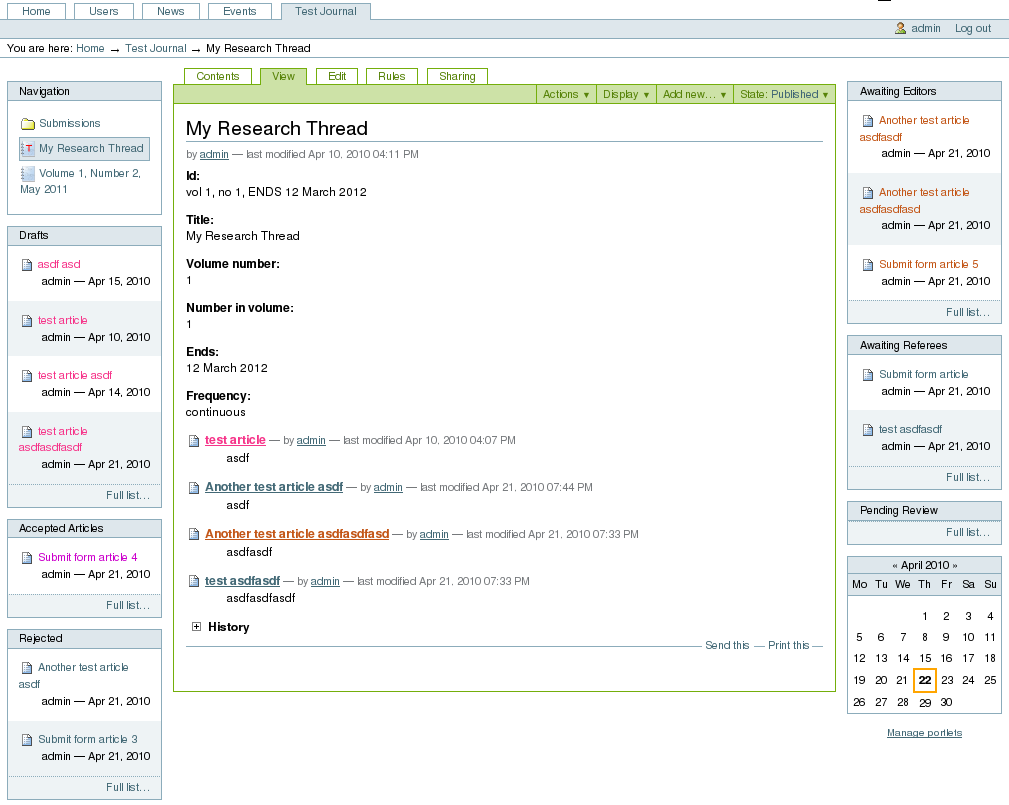
\includegraphics[width=4in]{8-testjCommons-researchThread.png}
\end{center}
\end{frame} 

%
%
%
\begin{frame}{Workflows}{Peer Reviewed}
\mycomment{workflows tell us what happens when a submission is made - all possible steps through which a submission can go through in order to be accepted, rejected, or signaled (categories with options - Whitworth \& Friedman, 2009, First Monday). 
 
Submission of projects and articles will be done via the website Each time the state of an article changes, authors will be automatically informed via email, while the details (article text, issue name, etc) are all automatically filled in by the software 
 
We will be able to see queues of articles in different stages (submitted, being reviewed by issue editors, being peer reviewed, accepted, rejected, signaled, etc) in boxes.
 
Each member can have a customised view of the entire website for example - an issues editor will be able to see only portlets (queues with articles in stages) to do with their issue.
\bigskip
{\bf Talk about Conference, plus variations}
}


\begin{center}
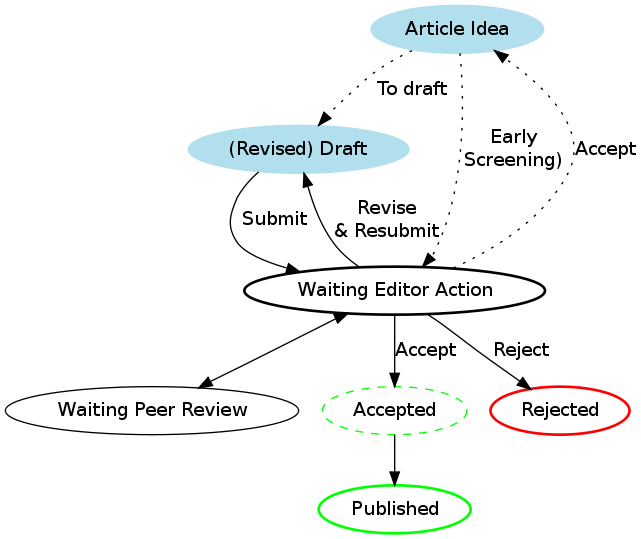
\includegraphics[width=3.5in]{WorkflowPR.png}
\end{center}
\end{frame}

\begin{frame}{Workflows}{Non Peer Reviewed}
\begin{center}
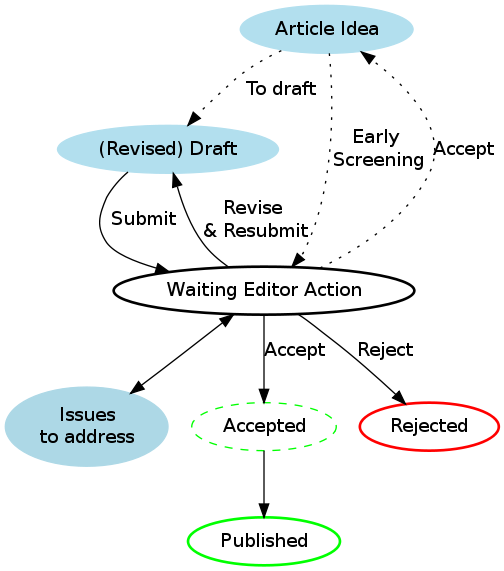
\includegraphics[width=2.7in]{WorkflowNonPR.png}
\end{center}
\end{frame}

\begin{frame}{Article queues/states}{}
\begin{center}
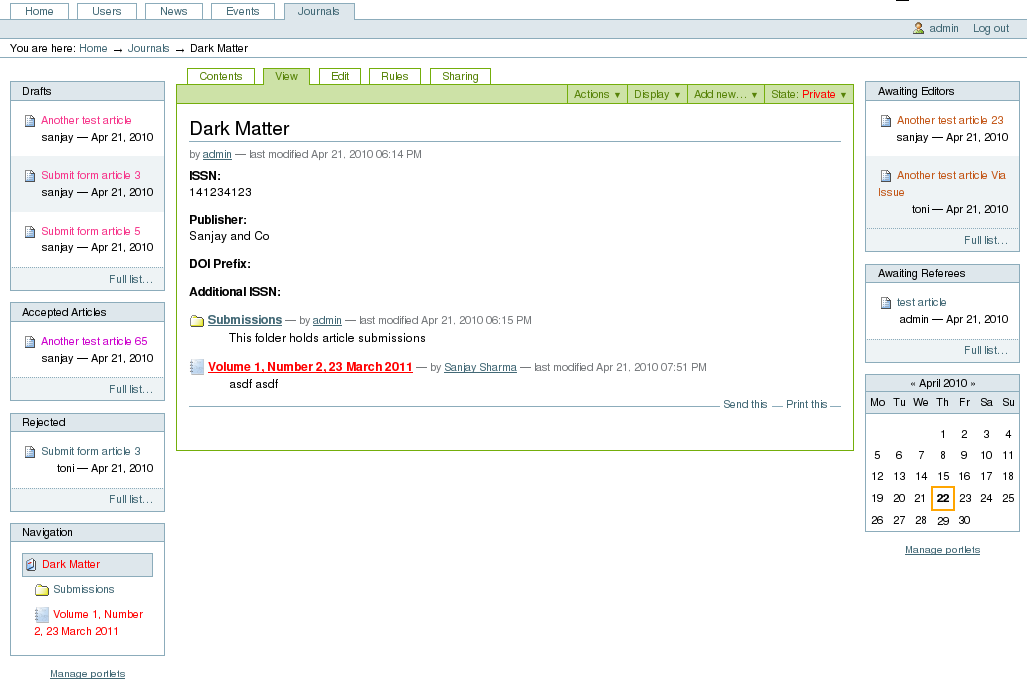
\includegraphics[width=4in]{5-darkmatter-ArticleQueues.png}
\end{center}
\end{frame} 

\begin{frame}{Article history}{}
\begin{center}
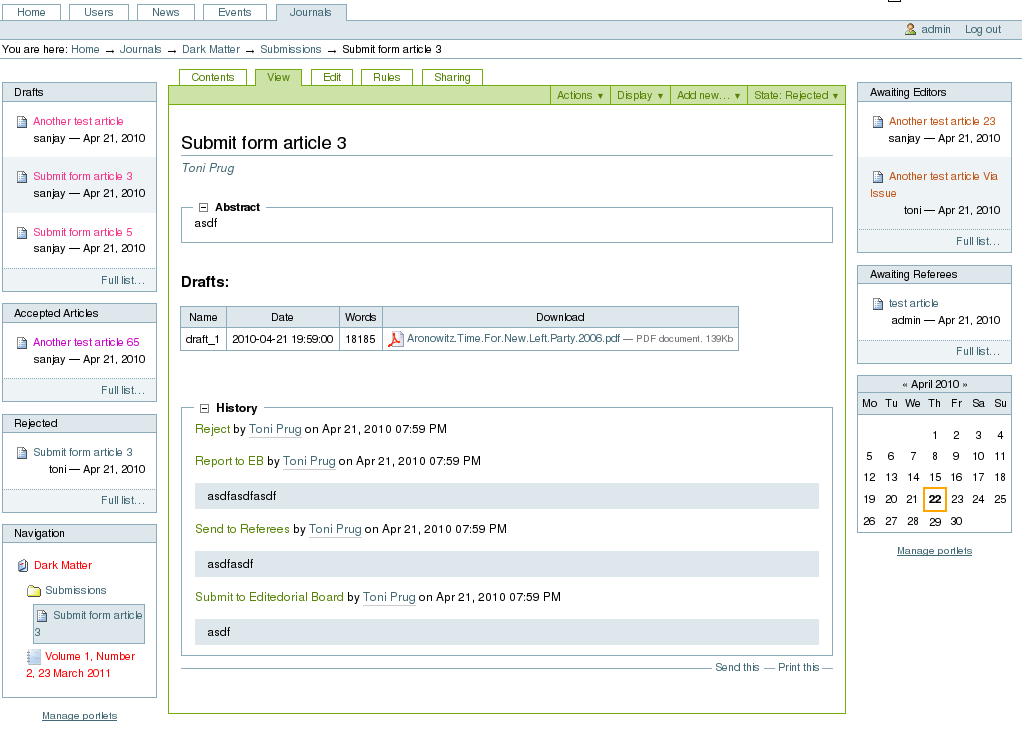
\includegraphics[width=4in]{6-darkmatter-ArticleHistory.png}
\end{center}
\end{frame} 


\begin{frame}{Submissions}{Track your work}

\begin{center}
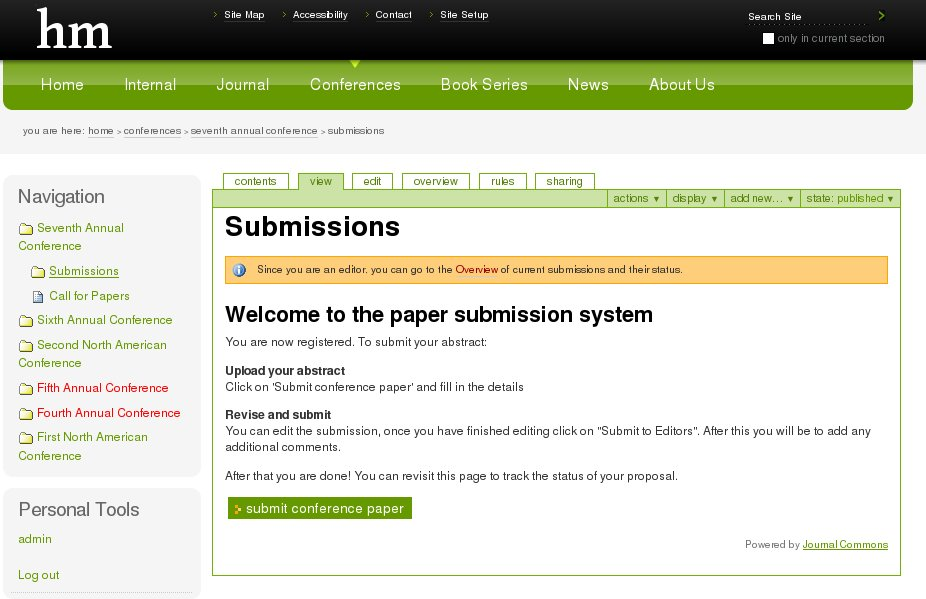
\includegraphics[width=4in]{1-conference-submissions-homepage.jpg}
\end{center}
  
\mycomment{Explain that Submissions come a bit from Poi (Issue Tracker, 
  Trouble Tickets) by status, by action, by responsible, by alarms (3 months...)
  }
\end{frame} 

\begin{frame}{Submissions}{Track your work}
\begin{center}
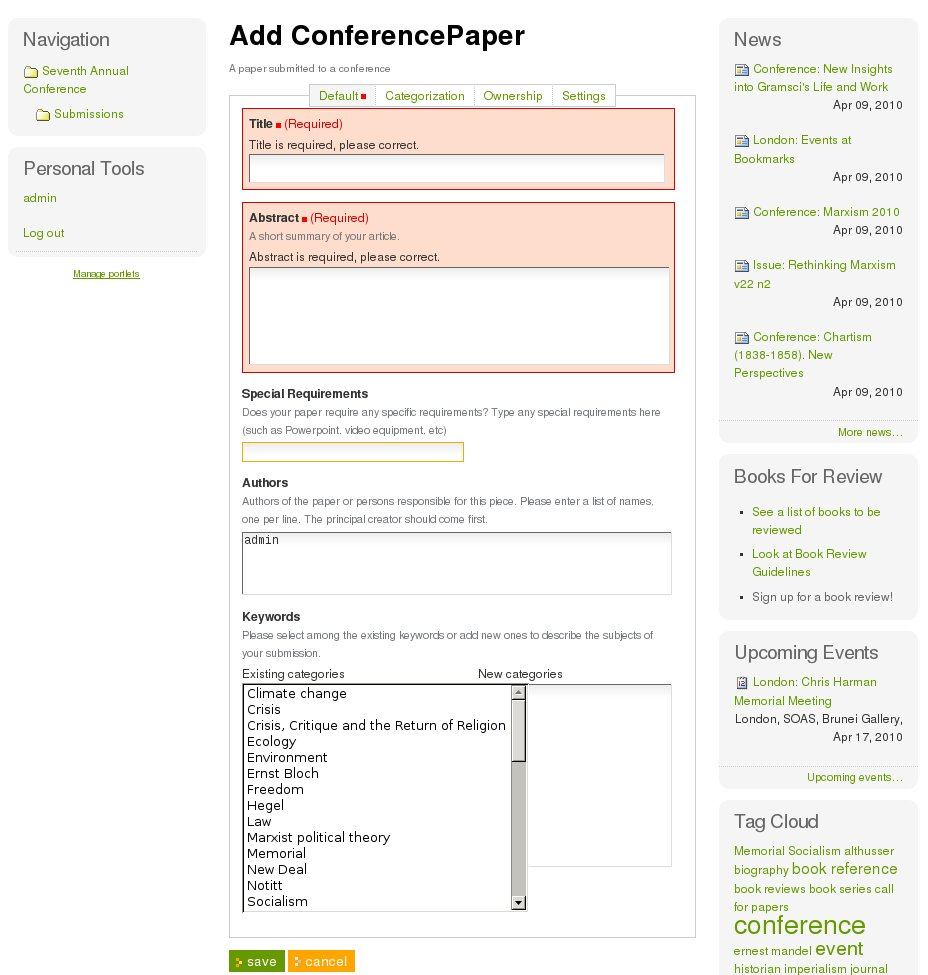
\includegraphics[width=4in]{2-conference-SubmitConferencePaper-form.jpg}
\end{center}
\end{frame} 

\begin{frame}{Submissions}{Track your work}
\begin{center}
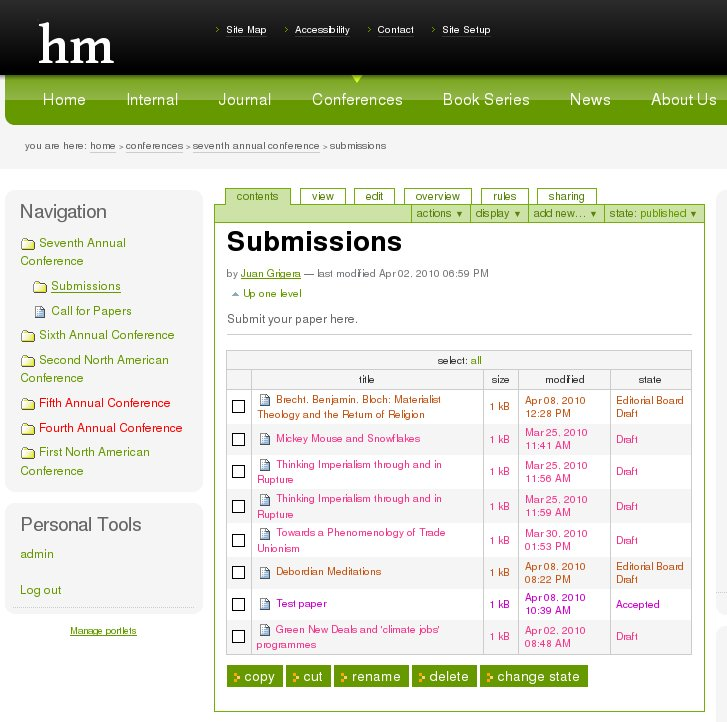
\includegraphics[width=3.5in]{3-conference-ListAllSubmissions.jpg}
\end{center}
\end{frame} 

\begin{frame}{Submissions}{Track your work}
\begin{center}
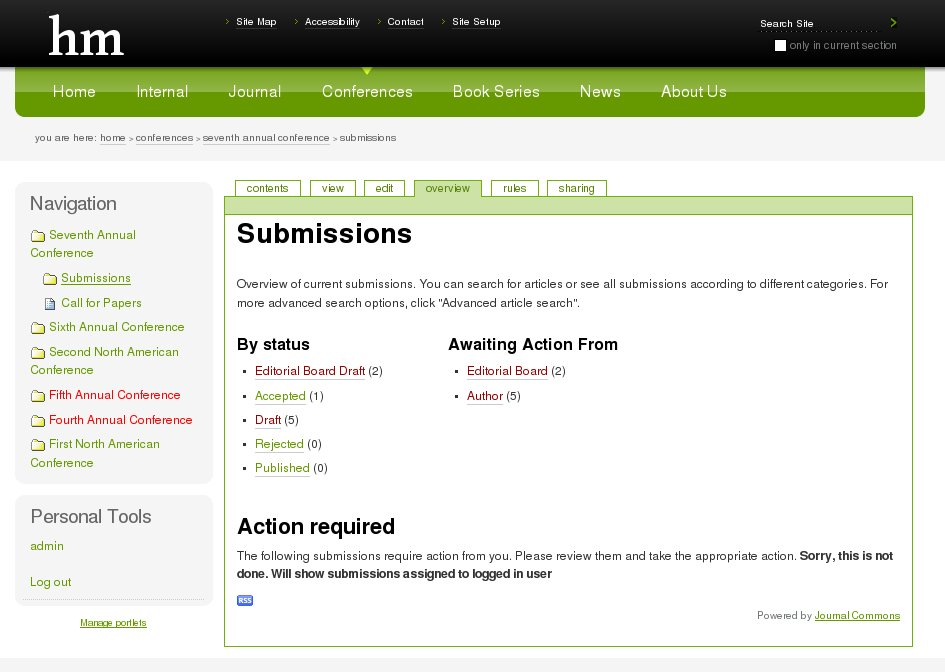
\includegraphics[width=4in]{4-conference-SubmissionsCategoriesAndActions.jpg}
\end{center}
\end{frame} 

\section{Shades of openness}

\begin{frame}{Contiuum of practices}
 
\begin{itemize}
\item Since whole process is on a website. Then {\bf opennes==ACLs}

\item We can accommodate everything from blind peer review, extend to CE/AB or open process (open process reviewing, early screening). 
Even publishing of arts works with some form of peer review (curating or collective models).

\item We can do it all simultaneously, using one collaborative-reviewing-publishing platform

\item We can even display articles/artsworks published through those different types of workflows with an icon (so that they can appear next to each other clearly distinguished) signifying: blind-peer-review, open-process peer review, semi-open-process, artwork-peer-reviewed, artwork-curated, etc. (PlaceableWorkflow and acquisition)
\end{itemize}
\end{frame}

\begin{frame}{Signals}

Signals are a way to choose a series of drop-down menu ratings, signaling to the reader on several aspects of the article, rather then using the binary publish/reject model. Fuzzy logic.

\begin{description}
\item [types] activist, academic, journalistic
 \mycomment{activist (article proposes a critique of a policy or practice with specific 
action proposals or suggestions), academic (article follows conventions of academic research article, position in literature, cited sources, and claimed contribution)}

\item [language quality] expression/narrative of article 
\item [logical flow] ideas are well organised in article
\item [originality] the argument presented in article is new
\item [evidence] there are many established arguments for which the most valuable contribution would be further and better evidence
\item [commendations] signal appreciation of the article. brief statement rather than a drop-down menu with options --- 50 words.
\end{description}

\scriptsize See
            [\href{http://www.oekonux.org/journal/list/archive/msg00233.html}{Discussion
                on Ratings/Signals}] And
            [\href{http://firstmonday.org/htbin/cgiwrap/bin/ojs/index.php/fm/article/view/2642/2287}{``Reinventing
                academic publishing online. Part I: Rigor, relevance
                and practice'', First Monday, Volume 14, Number 8 - 3
                August 2009; Whitworth B and R Friedman }]



\mycomment{Or perhaps recommended to others 1 (only to those with a very specific interest) to 10 (universal essential knowledge)}

\end{frame}

\section{Coding/dev}
\begin{frame}{issue tracker}{}
 \begin{center}
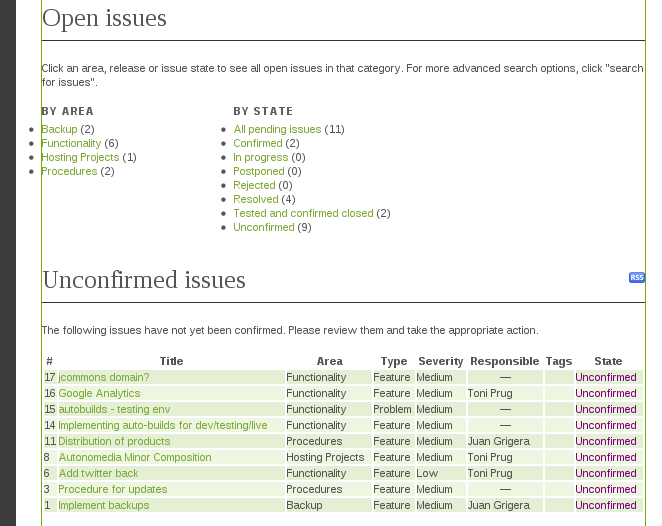
\includegraphics[width=3.5in]{10-tracker.png}
\end{center}
\end{frame}

\begin{frame}{source code}{}
 \begin{center}
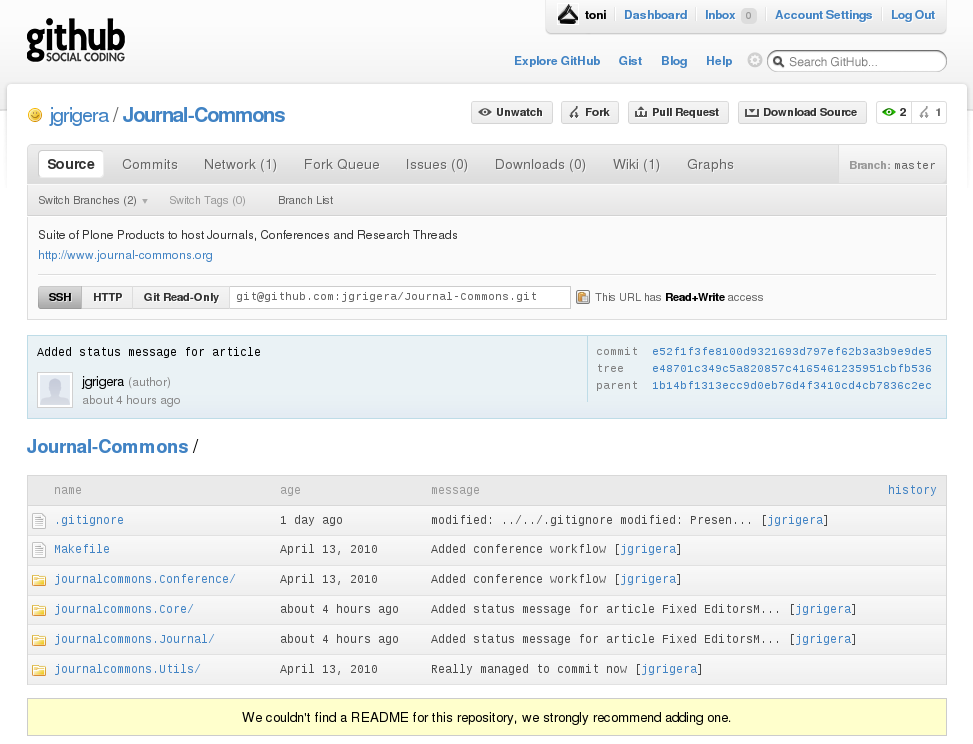
\includegraphics[width=4in]{11-github.png}
\end{center}
\end{frame}


\section{Further directions}
\begin{frame}{journalcommons}{}
 
\begin{itemize}
 \item {\tt COMING SOON ... www.journal-commons.org}
 \item Conference
 \item Lab
 \item Books (collaborative book publishing and editing platform)
\end{itemize}

\vfill

Early Funding: Cultural Studies Association of USA and School of
Business and Management, Queen Mary, University of London

\includegraphics[scale=0.5]{qm-logo.png}

\end{frame}
